\documentclass[12pt]{article}
\usepackage[utf8]{inputenc}
\usepackage[UTF8]{ctex}
\usepackage{biblatex}
\usepackage{amssymb}
\usepackage{latexsym}
\usepackage{amsmath}
\usepackage{cases}
\usepackage{geometry}
\usepackage{graphicx}
\usepackage{float}
\usepackage{listings}
\usepackage{enumerate}
\usepackage{color}
\usepackage{hw1}

% 调整目录间距的宏包
\usepackage{setspace}

\usepackage{multirow}
\usepackage{float}
\usepackage{fancyhdr}  % header,footer的设置

\newcommand{\subsubsubsection}[1]{\paragraph{#1}\mbox{}\\}
\setcounter{secnumdepth}{4} % how many sectioning levels to assign numbers to
\setcounter{tocdepth}{4} % how many sectioning levels to show in ToC

% 封面的相关命令设置
\newcommand{\hmwkTitle}{Project 7 Shooting method}
\newcommand{\hmwkClass}{《现代集成电路分析方法》}
\newcommand{\hmwkCompleteTime}{\today}
\newcommand{\hmwkAuthorName}{姓名:蔡志杰 }
\newcommand{\hmwMajor}{专业:电子科学与技术}
\newcommand{\hmwNumber}{学号:22112020002}
% 用fancyhdr设置header和footer
\pagestyle{fancy}
\lhead{\hmwkClass \hmwkTitle}
\rhead{蔡志杰 \quad 22112020002}
\cfoot{\thepage}


\addbibresource{bib.bib}
\setlength{\parindent}{0em}
\bibliography{bib}
\geometry{a4paper,scale=0.8}
\linespread{1.5}
\graphicspath{{Images/}}


%%%%%%%%%%%%%
%%% COVER %%%
%%%%%%%%%%%%%
\begin{document}

\begin{sloppypar}
\begin{titlepage}
\begin{center}
% \linespread{1.2}\huge {\bfseries Fudan University}\\[1cm]
% \linespread{1}
% \includegraphics[width=10cm]{fudan-name.pdf}\\[3cm]
% \linespread{1.9}\huge {\bfseries 可编程器件与硬件描述语言}\\
% \linespread{1.9}\LARGE {\bfseries 作业报告}\\[2.5cm]

% {\Large 姓名:名字}\\[0.3cm]
% \Large 学号:123456789\\[4cm] 
% \large 2021年11月1日



\includegraphics[scale = 0.9]{fudan.jpg}\\

\includegraphics[scale = 0.6]{fudan_logo.jpg}\\
\vspace{0.5in}
\linespread{1.9}\huge {\bfseries 现代集成电路分析方法}\\
\linespread{1.9}\LARGE {\bfseries \textbf{\hmwkTitle}}\\
\vspace{1.0in}
\large \hmwMajor{}\\
\large \hmwNumber{}\\
\large \hmwkAuthorName{}\\
% \large \date{\today} 

\end{center}
\end{titlepage}



%---------以下生成目录----------
\newpage
\begin{spacing}{1.2}
	\tableofcontents
\end{spacing}   % 若不想要目录, 注释掉该句
\thispagestyle{empty}   % 不要页眉页脚和页码
\newpage

%%%%%%%%%%%%%%%%%%%%%%%%%
%%% Problem Statement %%%
%%%%%%%%%%%%%%%%%%%%%%%%%
\section{题目}
\qquad 采用shooting method求解如下线性系统的周期稳态解:
\begin{equation}
\label{MNA}
C \dot{X}+G X=B U
\end{equation}
\begin{equation}
Y=L^T X 
\end{equation}

\subsection{输入}
\qquad 输入的线性电路为SPICE格式的网表文件 \par
\qquad (1)电路方程:以提供的stamp程序的输出作为本程序的输入。 \par
\qquad (2)输入u(t) = cos (200$\pi t$),也可以采用其他周期输入。 \par

\subsection{输出结果}
\qquad (1)通过shooting method求解得到的初值。 \par
\qquad (2)在求解的初值条件下,通过后向欧拉方法得到的周期稳态解\par

\subsection{测试用例}
\qquad Benchmark 目录下提供三个测试用例RLC\_s3.sp,bus32bit8seg.sp 以及bus8bit8seg.sp,并提供Matlab下的stamp程序供构造电路矩阵。stamp用法请参考Benchmark目录下的stamp\_man文件。\par

\subsection{提交结果}
\qquad 程序建议采用MATLAB完成,需提交以下内容: \par
\qquad (1) 源程序,应有必要的注释。 \par
\qquad (2) 使用除MATLAB外其他语言的,需要提交最终编译的可执行代码。 \par
\qquad (3) 一份完整的说明,主要内容包括:主要设计思想,程序结构,编译的环境和方法,运行的环境和方法,输入的格式或方法,以及其他需要特别说明的地方。 \par
\qquad (4) 对测试用例的测试结果和分析。 \par


%%%%%%%%%%%%%%%%%
%%% Algorithm %%%
%%%%%%%%%%%%%%%%%

\section{算法原理}

\qquad 首先通过stamp程序获得spice网表对应的电路MNA方程。对于周期性的输入激励信号系统一般会得到一个周期稳态解,使用前面基于有限差分的方法(前向、后向欧拉和梯形法)可以得到系统的稳定解,但是需要很大的预算量(从0时刻开始),因此可以采用Shooting法来求解周期稳态解的初始解,再基于这个初始解求解周期稳态解,或是使用谱方法将周期稳态解用一组基函数表示,再减小基函数线性组合后于原函数的残差来获得周期稳态解。

\qquad 本项目的整体思路是首先根据shooting method将周期性稳态信号转换成一个状态函数,并将周期信号在一个周期中收尾相等的约束转换成对一个函数零点的求解问题。之后使用牛顿法来迭代前面构造的函数零点,进而求解周期信号的初值。最后根据求解得到的初值再使用后向欧拉来求解在周期激励信号的作用下系统的周期稳态解。接下来将分别介绍整个框架中涉及到的算法,包括Shooting method,牛顿迭代法,后向欧拉法和广义共轭残差法。\par


\subsection{Shooting Method}
\qquad Shooting method以瞬态分析为基础直接在时域中求解电路的周期稳态响应,求解的方法则是令一个周期起始与终止点中电路的状态一致,即$x(0) = x(T)$,可以通过牛顿迭代法来不断减小误差,让其小于一定的误差容限$|x(T)-x(0)| < \xi$进而得到一个初始解。假设状态变量为$x(t)$,电路方程为$C\frac{dx(t)}{dt}+Gx(t)=BU(t)$。假设电路激励信号的周期为T,当电路达到稳定状态时应满足$x(0) = x(T)$。为了能够使用牛顿迭代法进行求解,构造状态转换函数$\phi(y,t_0,t_1) = x(t_1)$。其含义是,对于$x(t_0)=y$的情况,$t_1$时刻的状态值$x(t_1)$等于$\phi(y,t_0,t_1)$。进而初值求解问题可以转换成求解下面函数零点的问题:
\begin{equation}
  H(x(0)) = \phi(x(0),0,T) - x(0)
\end{equation}
\qquad 使用牛顿迭代法对该函数零点进行求解可以得到迭代公式$H\left(x^k\right)+J_H\left(x^k\right)\left(x^{k+1}-x^k\right)=0$,$J_H\left(x^k\right)\left(x^{k+1}-x^k\right)=-H\left(x^k\right)$。其中$J_H$为$H(x)$的Jacobi矩阵:
\begin{equation}
  J_H(x)=\frac{\partial H(x)}{\partial x}=\frac{\partial(\phi(x, 0, T))-x}{\partial x}=\frac{\partial(\phi(x, 0, T))}{\partial x}-I
\end{equation}

\qquad 为了求解牛顿迭代法的Jacobi矩阵,采用后向欧拉法中的思路,首先将整个周期T等分为L个区间,$\Delta t = \frac{T}{L}$,此时由后向欧拉可得:

\begin{equation}
  C \frac{x_{l+1}-x_l}{\Delta t}  + G x_{l+1}= BU(t_{l+1}) 
\end{equation}

\qquad 等式两边对$x_l$求导可得:
\begin{equation}
  C \frac{\partial x_{l+1}}{\partial x_{l}} - C \frac{\partial x_l}{\partial x_{l}}  + \Delta t G\frac{\partial x_{l+1}}{\partial x_{l}} = \Delta t \frac{\partial BU(t_{l+1})}{\partial x_{l}} = 0
\end{equation}

\qquad 整理可得下式,对任意$l \in [0,L-1]$成立:

\begin{equation}
  \frac{\partial x_{l+1}}{\partial x_{l}} = C(C+\Delta t G)^{-1}
\end{equation}

\qquad 因此可得:

\begin{equation}
  \frac{\partial(\phi(x, 0, T))}{\partial x} = \prod_{l=0}^{L-1} \frac{\partial x_{l+1}}{\partial x_{l}} = \prod_{l=1}^L C\left(C+G_{\Delta} t\right)^{-1}=\left(C\left(C+G_{\Delta} t\right)^{-1}\right)^L
\end{equation}

\qquad 进而得到Jacobi矩阵:
\begin{equation}
  J_H(x) = \frac{\partial(\phi(x, 0, T))}{\partial x} - I = \left(C\left(C+G_{\Delta} t\right)^{-1}\right)^L - I
\end{equation}

\qquad 因此牛顿迭代公式为:
\begin{equation}
  \left(\left(C\left(C+G_{\Delta} t\right)^{-1}\right)^L - I \right) \left(x^{k+1}-x^k\right)=-H\left(x^k\right) = x^k - \phi(x^k,0,T)
\end{equation}

\qquad 迭代求解时先设定初值,然后根据迭代公式进行迭代,直到两轮迭代结果小于误差容限且函数值的绝对值也小于误差容限时停止迭代。

\qquad 得到初始解后可以通过后向欧拉方法根据电路初值求解电路响应,后向欧拉的求解方法将在\ref{BE}节进行介绍。

\subsection{牛顿迭代法}
\qquad 牛顿迭代法是求解非线性方程的一种方法,其最大优点是在方程的单根附近具有平方收敛,而且该法还可以用来求方程的重根、复根,此时线性收敛,但是可通过一些方法变成超线性收敛。其主要思路是通过将非线性方程$f(x) = 0$用线性近似(泰勒展开),进而得以进行求解。忽略二次及以上的高阶项后泰勒展开的结果如下:
\begin{equation}
  0=f\left(x^*\right) \cong f\left(x^k\right)+\frac{d f}{d x}\left(x^k-x^*\right)
\end{equation}

\qquad 其中$x^*$为准确解,$x^k$为第k次迭代结果,上式整理后可得如下的迭代公式:

\begin{equation}
  x^{k+1}=x^k-\left[\frac{d f}{d x}\left(x^k\right)\right]^{-1} f\left(x^k\right)
\end{equation}

\qquad 收敛条件为$\left|\left[\frac{d f}{d x}(x)\right]^{-1} \frac{d^2 f}{d^2 x}(x)\right| \leq L$其中L为有界的常数,即$\frac{d f}{d x}(x)$不收敛于0,$\frac{d^2 f}{d^2 x}(x)$不趋于无穷。此外为了保证较好的收敛性还需要一个较好的初值同时需要两个收敛条件来防止错误的收敛:

\begin{equation}
  \left\|x^{k+1}-x^k\right\|<\varepsilon_{x_\alpha} , \qquad \left\|f\left(x^{k+1}\right)\right\|<\varepsilon_{f_\alpha}
\end{equation}


\subsection{后向欧拉法Backward Euler}\label{BE}
\qquad 后向欧拉法为有限差分法的一种,通过对时间的离散化以及使用差分来逼近微分的方法求解一阶偏微分方程。对于如下的偏微分方程,使用时间上更早的数据点做差分来逼近梯度,具体公式如下。

\begin{equation}
  \frac{dx(t)}{dt}=Ax(t) 
\end{equation}
\begin{equation}
  x(t_0) = x_0
\end{equation}

\begin{equation}
\frac{d}{d t} x\left(t_{l+1}\right)=A x\left(t_{l+1}\right) \cong \frac{x\left(t_{l+1}\right)-x\left(t_l\right)}{\Delta t}
\end{equation}
\begin{equation}
x\left(t_{l+1}\right) \cong x\left(t_l\right)+\Delta t A x\left(t_{l+1}\right)
\end{equation}
公式\ref{MNA}中后向欧拉的迭代公式为:
\begin{equation}
    (C+\Delta tG)X(t_{l+1}) = CX(t_{l}) + \Delta t BU(t_{l+1})
\end{equation}


\subsection{广义共轭残差法GCR}
\qquad 广义共轭残差法是求一种解线性方程组的方法,通过残差来决定每次的探索方向,每次探索方向之间彼此正交来保证每次搜索时目标函数的最优性。对于线性方程组$Mx=b$,广义共轭残差的求解原理如下。
\qquad 第$k$轮残差的定义为,$ r^k \equiv b - Mx^k$, 第k轮迭代的解$x_k$定义为,$x^{k+1} = \sum_{i=0}^{k} \alpha_i w_i$, 目标是最小化残差的2范数。当构成$x$的基向量关于$M$矩阵正交,即$(Mw_i)^T(Mw_j)=0 (i \neq j)$时残差的2范数很容易优化,
\begin{equation}
  \mathop{\min}_{x} \Vert r^{k+1} \Vert_2^2 = \Vert b - \sum_{i=0}^{k} \alpha_i M w_i \Vert
\end{equation}
\qquad 将其转换成一个二次型目标函数,取最优值的地方梯度为0,梯度对应的就是残差,能够间接求解线性方程组。(只适用于矩阵$M$为对称正定阵)
\begin{equation}
  f(x) = \frac{1}{2}x^TMx-x^Tb
\end{equation}
\begin{equation}
  \triangledown_xf(x) = Mx-b
\end{equation}
\qquad 对目标函数f采用最速下降法,将梯度作为新的探索方向,经过分析可得如下的迭代公式:
\begin{equation}  
  \alpha_k= \frac{\left(r^k\right)^T\left(M p_k\right)}{\left(M p_k\right)^T\left(M p_k\right)} 
\end{equation}
\begin{equation}
  x^{k+1} =x^k+\alpha_k p_k
\end{equation}
\begin{equation}
  r^{k+1} =b-M x^{k+1} =b-M x^k-\alpha_k M p_k =r^k-\alpha_k M p_k
\end{equation}
\begin{equation}
  p_{k+1} =r^{k+1}-\sum_{j=0}^k \frac{\left(M r^{k+1}\right)^T\left(M p_j\right)}{\left(M p_j\right)^T\left(M p_j\right)} p_j
\end{equation}
\qquad 如果矩阵$M$是稀疏的,具有$k$个特征值,你们只需要$k$轮迭代即可收敛,收敛速度更快。当矩阵$M$为对称矩阵时,$r^{k-1} \bot Mp_j,j<k$,$p_{k+1}$的正交化只需要一步操作。
\begin{equation}
  p_{k+1}=r^{k+1}-\sum_{j=0}^k \frac{\left(M r^{k+1}\right)^T\left(M p_j\right)}{\left(M p_j\right)^T\left(M p_j\right)} p_j \Rightarrow p_{k+1}=r^{k+1}-\frac{\left(M r^{k+1}\right)^T\left(M p_k\right)}{\left(M p_k\right)^T\left(M p_k\right)} p_k
\end{equation}

\section{算法实现}

\subsection{算法流程}
\qquad 算法流程
\begin{itemize}
  \item 使用提供的stamp动态库对hsipce网表进行解析得到相应的矩阵数据,使用hspice进行仿真,得到相应的波形lis文件,调用read\_data函数来得到相应lis文件中hspice仿真的波形结果。(main.m)
  \item 根据stamp解析到的输入信号信息生成相应的激励信号数和相应的信号周期。(GenerateSrc.m)
  \item 根据函数的输入参数决定shooting method的分段数L和牛顿迭代法的最大轮数和误差,并进行初值的求解。(main.m)
  \item 使用后向欧拉根据初值求解微分方程。(BackwardEuler.m)
  \item 上面求解过程中需要对线性方程组求解的地方提供了两种求解的方法:matlab自带的“$\backslash$”和自己实现的GCR(Golden.m,GCR.m)
  \item 将得到的仿真结果通过线性插值得到与hspice相同采样时间的数据点,并计算相应的误差(最大绝对误差和均方绝对误差)。(main.m)
  \item 生成结果对比图。(report.m)
\end{itemize}

\subsection{输入激励信号}
\qquad 脉冲源

\qquad 语法:

\qquad Vxxx n+ n- PU<LSE> <(>v1 v2 <td <tr <tf <pw <per> > > > > <)>

\qquad Ixxx n+ n- PU<LSE> <(>v1 v2 <td <tr <tf <pw <per> > > > > <)>

\qquad 其中v1为脉冲源的低压,v2为高压,td为延迟,tr为上升时间,tf为下降时间,pw为脉冲宽度,per为信号周期。下图展示了一个脉冲信号源的例子:

\begin{figure}[H]
  \centering
  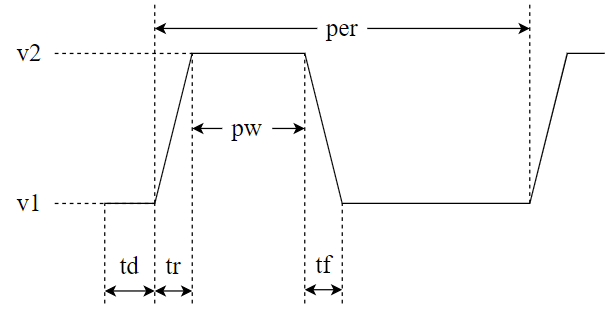
\includegraphics[width=0.5\columnwidth]{figure/pulse.png}
  \caption{脉冲信号源示例}
\end{figure}

\qquad 正弦源

\qquad 语法:

\qquad Vxxx n+ n- SIN <(> vo va <freq <td <$\theta$ <$\phi$>>>> <)>

\qquad Ixxx n+ n- SIN <(> vo va <freq <td <$\theta$ <$\phi$>>>> <)>

\qquad 其中vo为直流幅度,va为交流幅度,freq为频率,td为延时,$\theta$为衰减因子,$\phi$为相位延时。信号的公式可以如下:

\begin{equation}
  y(t) = e^{-\theta}\cdot va \cdot sin(2\pi freq \cdot(t-td) - \phi) + vo
\end{equation}


\subsection{输出}
\qquad 为了将仿真结果与hspice的结果进行对比,首先需要通过插值法得到自己仿真结果在hspice采样时间上的值,然后求解最大绝对误差和均方绝对误差。同时为了方便访问结果,使用save命令将仿真的数据存储到.mat文件中(文件在Benchmark目录下,文件命名与图中对应图注相同)。对于有多个输出节点的电路,为了方便观察选取其中一个的波形进行绘制。

\subsection{编译与运行}
\qquad 程序基于Matlab 2015b(32位)平台,将整个解析网表文件, shooting method过程和结果输出的过程都打包在main函数中,由于所有benchmark都在Benchmark目录中,所以需要在matlab中将当前目录切换到Benchmark下运行。main函数的接口为$main(caseName, L, \\ newtonMaxIter, newtonErrorThres, errorThres)$.其中caseName(RCL\_s3(正弦信号作为激励),RCL\_p3(方波信号作为激励),bus8bit8seg(正弦信号作为激励),bus8bit8seg\_p(方波信号作为激励),bus32seg16(正弦信号作为激励),bus32seg16\_p(方波信号作为激励))。L为Shooting的分段数,newtonMaxIter, newtonErrorThres为牛顿迭代法中的最大迭代轮数和两个误差容限(两个误差容限放在一个向量变量中),errorThres为GCR的误差阈值。下面给出一个运行示例:

\begin{equation}
  main('RLC_s3',50,50,[1e-9, 1e-9],1e-9)
\end{equation}

\section{结果与分析}
\subsection{实验结果}

\subsubsection{RLC电路}
\subsubsubsection{正弦激励}

\qquad 仿真设置:牛顿迭代法的最大迭代轮数为50轮,同时两个误差容限都为$1e^{-9}$,采用matlab自带线性方程组求解方法,shooting的分段数量为50,输入的正弦信号为$sin(200\pi t)$,仿真的时间为0-20ms,采样时间间隔为0.004ms。shooting得到的初值为:$x_0$=[-0.0000,-0.1699,-0.0693,-0.0733,-0.1267,-0.1300,-0.1675,0.0198,0.0198,0.0153,0.0107]。下图为仿真结果:

\begin{figure}[H]
  \centering
  \includegraphics[width=0.7\columnwidth]{figure/RLC\_s3\_golden.png}
  \caption{RLC\_s3\_golden仿真结果}
\end{figure}

\qquad 从结果中可以看出由于直接使用了shooting得到的初值,在刚开始的一段时间内与hspice得到的结果误差较大,这是由于hspice的结果考虑了电路稳态的建立过程,而基于shooting得到的结果则直接得到周期稳态解,随着时间的推进初始解分量不断衰落,可以看出仿真结果与hspice仿真结果的误差变小。下图绘制了电路稳定后的一段时间内(10ms-20ms)的仿真结果,也可以印证前面的结论。

\begin{figure}[H]
  \centering
  \includegraphics[width=0.7\columnwidth]{figure/RLC\_s3\_partial.png}
  \caption{RLC\_s3\_partial仿真结果}
\end{figure}

\subsubsubsection{方波信号激励}

\qquad 仿真设置:牛顿迭代法的最大迭代轮数为50轮,同时两个误差容限都为$1e^{-9}$,采用matlab自带线性方程组求解方法,shooting的分段数量为50。输入的方波信号为周期为8ms,高低电平分别为3V和0V,上升下降时间为0.5ms,高电平时间为3ms,信号延迟为1ms。仿真的时间为0-20ms,采样时间间隔为0.004ms。shooting得到的初值为:$x_0$=1.0e-03 * [0,0.3100,0.1340,0.1340,0.2373,0.2373,0.3100,-0.0383,-0.0383,-0.0295,-0.0208]。下图为仿真结果,绝对误差同样也体现了初始解分量的衰减。

\begin{figure}[H]
  \centering
  \includegraphics[width=0.7\columnwidth]{figure/RLC\_p3\_golden.png}
  \caption{RLC\_p3\_golden实验结果}
\end{figure}


\subsubsection{bus8bit8seg电路}
\subsubsubsection{正弦激励}

\qquad 仿真设置:牛顿迭代法的最大迭代轮数为50轮,同时两个误差容限都为$1e^{-9}$,采用matlab自带线性方程组求解方法,shooting的分段数量为50。输入的正弦信号为$sin(200\pi t)$。仿真的时间为0-3e-8s,采样时间间隔为1e-11s。由于解的维度过大(有250个节点)只展示前十个初始解$x_0(1:10)$=[0.0733,-0.0159,-0.0057,-0.0052,-0.0051,-0.0050,-0.0050,-0.0050,-0.0017,-0.0010]。下图为仿真结果:

\begin{figure}[H]
  \centering
  \includegraphics[width=0.7\columnwidth]{figure/bus8bit8seg\_golden.png}
  \caption{bus8bit8seg\_golden实验结果}
\end{figure}

\qquad 采用自己实现的GCR算法进行线性方程组的求解(误差容限1e-9)得到如下的结果(除了线性方程组的求解方法变化外,其余部分与上面设置相同)。从结果可以看出使用GCR的运行速度比使用matlab自带的求解器慢了很多,整个shooting过程的运行时间增加了两个数量级(1.7s->279.5s),但是计算得到的误差是相同的,这说明了实现的GCR算法功能是正确的,但是在计算效率上和matlab自带的还有很大的差距。

\begin{figure}[H]
  \centering
  \includegraphics[width=0.7\columnwidth]{figure/bus8bit8seg\_gcr.png}
  \caption{bus8bit8seg\_gcr实验结果}
\end{figure}

\subsubsubsection{方波信号激励}

\qquad 仿真设置:牛顿迭代法的最大迭代轮数为50轮,同时两个误差容限都为$1e^{-9}$,采用matlab自带线性方程组求解方法,shooting的分段数量为50。输入的方波信号为周期为1e-8s,高低电平分别为3V和0V,上升下降时间为0.5e-9s,高电平时间为4e-9s,信号延迟为1e-9s。仿真的时间为0-3e-8s,采样时间间隔为1e-11s。由于解的维度过大(有250个节点)只展示前十个初始解$x_0(1:10)$=[0,0,0,0,0,0,0,0,0,0]。下图为仿真结果:

\begin{figure}[H]
  \centering
  \includegraphics[width=0.7\columnwidth]{figure/bus8bit8seg\_p\_golden.png}
  \caption{bus8bit8seg\_p\_golden实验结果}
\end{figure}

\qquad 采用自己实现的GCR算法进行线性方程组的求解(误差容限为1e-9)得到如下的结果(除了线性方程组的求解方法变化外,其余部分与上面设置相同)。从结果同样可以看出使用GCR的运行速度比使用matlab自带的求解器慢了很多,整个shooting过程的运行时间增加了两个数量级(1.7s->280.1s),但是计算得到的误差是相同的,同样说明了实现的GCR算法功能是正确的,但是在计算效率上和matlab自带的还有很大的差距。

\begin{figure}[H]
  \centering
  \includegraphics[width=0.7\columnwidth]{figure/bus8bit8seg\_p\_gcr.png}
  \caption{bus8bit8seg\_p\_gcr实验结果}
\end{figure}

\subsubsection{bus32seg16电路}
\subsubsubsection{正弦激励}

\qquad 仿真设置:牛顿迭代法的最大迭代轮数为50轮,同时两个误差容限都为$1e^{-9}$,采用matlab自带线性方程组求解方法,shooting的分段数量为50。8个电流源都输入$sin(200\pi t)$的正弦信号。仿真的时间为0-3e-8s,采样时间间隔为1e-11s。由于解的维度过大(有1666个节点)只展示前十个初始解$x_0(1:10)$=[0.3963,0.3777,0.3771,0.3770,0.3768,0.3766,0.3767,0.3948,-0.1089,-0.1092]。下图为仿真结果:

\begin{figure}[H]
  \centering
  \includegraphics[width=0.7\columnwidth]{figure/bus32seg16\_golden.png}
  \caption{bus32seg16\_golden实验结果}
\end{figure}


\subsubsubsection{方波信号激励}

\qquad 仿真设置:牛顿迭代法的最大迭代轮数为50轮,同时两个误差容限都为$1e^{-9}$,采用matlab自带线性方程组求解方法,shooting的分段数量为50。8个电流源都输入方波信号,详细设置:周期为1e-8s,高低电平分别为3V和0V,上升下降时间为0.5e-9s,高电平时间为4e-9s,信号延迟为1e-9s。仿真的时间为0-3e-8s,采样时间间隔为1e-11s。由于解的维度过大(有1666个节点)只展示前十个初始解$x_0(1:10)$=[0,0,0,0,0,0,0,0,0,0]。下图为仿真结果:

\begin{figure}[H]
  \centering
  \includegraphics[width=0.7\columnwidth]{figure/bus32seg16\_p\_golden.png}
  \caption{bus32seg16\_p\_golden实验结果}
\end{figure}

\subsection{结果分析}

\qquad 从结果中可以看出对于输入正弦激励信号的情况,由于直接使用了shooting得到的初值,在刚开始的一段时间内与hspice得到的结果误差较大,这是由于hspice的结果考虑了电路稳态的建立过程,而基于shooting得到的结果则直接得到周期稳态解,随着时间的推进初始解分量不断衰落,可以看出仿真结果与hspice仿真结果的误差变小。但是对于输入方波的情况刚输入的误差并不大,分析原因为方波信号有一定的延时,故起始的输出也都为0,和hspice接近。

\qquad 此外对比了使用自己实现的GCR算法matlab自带“反除操作$\backslash$”的进行线性方程组的求解。从结果可以看出使用GCR的运行速度比使用matlab自带的求解器慢了很多,整个shooting过程的运行时间增加了两个数量级,但是计算得到的误差是相同的。这说明了实现的GCR算法功能是正确的,但是在计算效率上和matlab自带的还有很大的差距。

\section{文件结构}
\begin{itemize}
  \item main.m:包含整个shooting method求解初值和基于初值求解电路方程响应的框架和流程。
  \item BackwardEuler.m:实现后向欧拉求解法。
  \item GCR.m:实现GCR算法。
  \item Golden.m:调用matlab自带的反除操作(“$\backslash$”用于线性方程)。
  \item GenerateSrc.m:生成激励信号和并返回信号周期。
  \item report.m:分析数据并绘制对比图。
\end{itemize}

\end{sloppypar}
\end{document}